\documentclass[pdftex,12pt,a4paper]{article}
\usepackage{tikz}
\usetikzlibrary{positioning}
\begin{document}

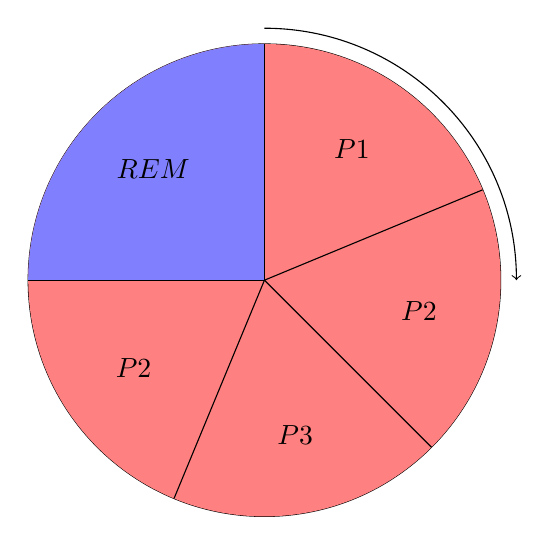
\begin{tikzpicture}
%  \draw[step=.5cm,gray,very thin] (-3,-3) grid(3,3);	% for debug
  \draw (0,0) circle (3);
  \def\r{3};
  \fill[red!50] (0,0) circle(\r);
  \fill[blue!50] (0,0) -- (90:3) arc[radius=\r, start angle=90, end angle=180] (180:3) -- cycle;
  % separator
  \foreach \a in {90, 22.5, -45.0, -112.5, -180} {
    \draw (0,0) -- (\a:\r);
  };
  % node
  \foreach \a in {90, 22.5, -45.0} {
    \def\i{\pgfmathparse{int((-\a+90)/67.5+1)}\pgfmathresult};
    \draw (\a-33.75:\r*2/3) node{$P\i$};
  };
  \draw(-112.5-33.75:\r*2/3) node {$P2$};
  \draw (90+45:\r*2/3) node {$REM$};
  % arrow
  \draw[->] (90:\r+.2) arc[radius=\r+.2, start angle=90, end angle=0];
\end{tikzpicture}

\vspace{1cm}

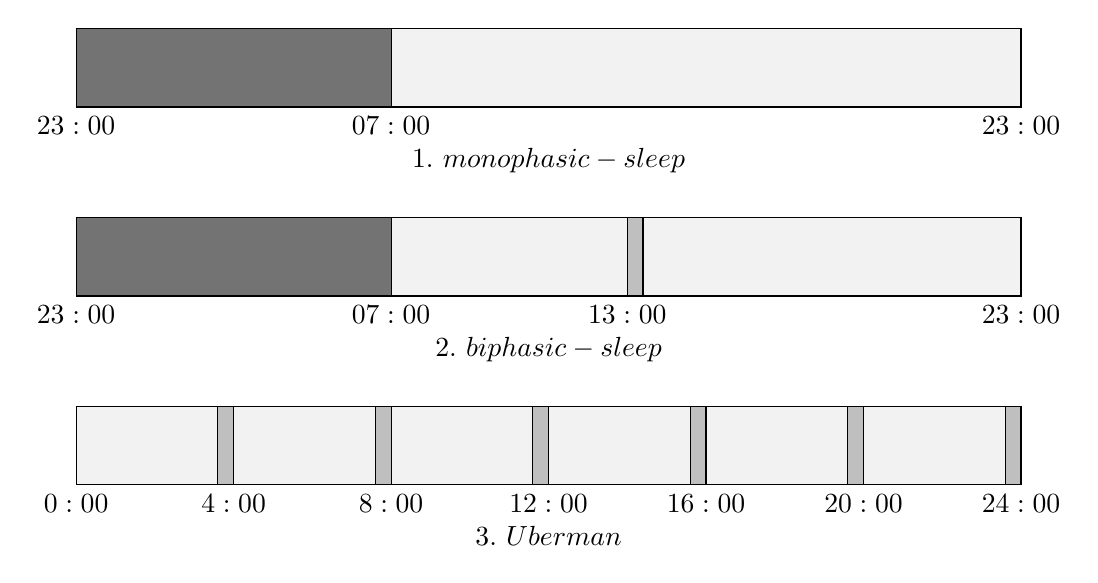
\begin{tikzpicture}[every node/.style={below}]
  \def\len{12}
  %pic1
  \coordinate (clock23) at (0,0);
  \coordinate (clock0) at (\len/24,0);
  \coordinate (clock7) at (\len*8/24, 0);
  \coordinate (clock13) at (\len*14/24, 0);

  \filldraw[fill=black!5] (0,0) rectangle (\len,1);
  % fill
  \filldraw[fill=black!55] (0, 0) rectangle (\len*8/24,1);
  % node
  \draw (clock23) node{$23:00$};
  \draw (clock7) node{$07:00$};
  \draw (\len, 0) node{$23:00$};
  \tikzset{yshift=-0.4cm}
  \draw (\len/2,0) node{$1.\ monophasic-sleep$};

  % pic2
  \tikzset{yshift=-2cm}
  \coordinate (clock23) at (0,0);
  \coordinate (clock0) at (\len/24,0);
  \coordinate (clock7) at (\len*8/24, 0);
  \coordinate (clock13) at (\len*14/24, 0);

  \filldraw[fill=black!5] (0,0) rectangle (\len,1);
  % fill
  \filldraw[fill=black!55] (0, 0) rectangle (\len*8/24,1);
  \filldraw[fill=black!25] (clock13) rectangle +(.2, 1);
  % node
  \draw (clock23) node{$23:00$};
  \draw (clock7) node{$07:00$};
  \draw (clock13) node{$13:00$};
  \draw (\len, 0) node{$23:00$};
  \tikzset{yshift=-0.4cm}
  \draw (\len/2,0) node{$2.\ biphasic-sleep$};

  % pic 3
  \tikzset{yshift=-2cm}
  \filldraw[fill=black!5] (0,0) rectangle (\len,1);

  \foreach \i in {1,...,6} {
    \def\pos{\i*\len*4/24}
    \def\nod{\pgfmathparse{int(\i*4)}\pgfmathresult:00}

    \filldraw[fill=black!25] (\pos, 0) rectangle +(-0.2,1);
    \draw (\i*\len/6, 0) node[below]{$\nod$};
  }
  \draw (0, 0) node{$0:00$};
  \tikzset{yshift=-0.4cm}
  \draw (\len/2,0) node{$3.\ Uberman$};
\end{tikzpicture}

\vspace{1cm}

% triphasic1-sleep
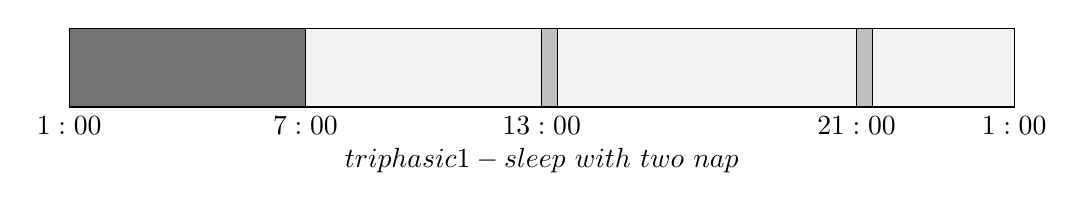
\begin{tikzpicture}[every path/.style={fill=black!25}, every node/.style={below}]
  \def\len{12}
  \filldraw[fill=black!5] (0,0) rectangle (\len, 1);

  \foreach \p in {1, 7, 13, 21} {
    \pgfmathparse{int((\p-1)*\len/24)}
    \draw (\pgfmathresult, 0) node {$\p:00$};
  }
  \draw (\len,0) node {$1:00$};
  \filldraw[fill=black!55] (0*\len/24, 0) rectangle (6*\len/24, 1);
  \filldraw (12*\len/24, 0) rectangle +(.2, 1);
  \filldraw (20*\len/24, 0) rectangle +(.2, 1);

  \tikzset{yshift=-.4cm}
  \draw (\len/2, 0) node{$triphasic1-sleep\ with \ two \ nap$};
\end{tikzpicture}

\vspace{1cm}

% triphasic2-sleep
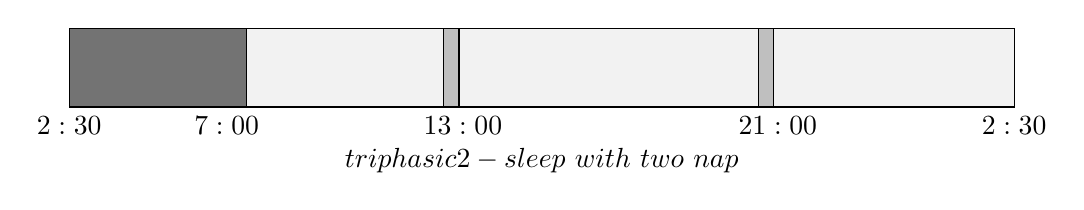
\begin{tikzpicture}[every path/.style={fill=black!25}, every node/.style={below}]
  \def\len{12}
  \filldraw[fill=black!5] (0,0) rectangle (\len, 1);

  \foreach \p in {7, 13, 21} {
    \pgfmathparse{int((\p-2.5)*\len/24)}
    \draw (\pgfmathresult, 0) node {$\p:00$};
  }
  \draw (\len,0) node {$2:30$};
  \draw (0,0) node {$2:30$};
  \filldraw[fill=black!55] (0*\len/24, 0) rectangle (4.5*\len/24, 1);
  \filldraw (9.5*\len/24, 0) rectangle +(.2, 1);
  \filldraw (17.5*\len/24, 0) rectangle +(.2, 1);

  \tikzset{yshift=-.4cm}
  \draw (\len/2, 0) node{$triphasic2-sleep\ with \ two \ nap$};
\end{tikzpicture}

\end{document}